\documentclass{beamer}
\usepackage[size=custom, width=21, height=27, scale=1.0, orientation=portrait]{beamerposter}
\setbeamertemplate{navigation symbols}{}
\setbeamersize{text margin left=0em,text margin right=0em}

\usepackage{tikz}
\usetikzlibrary{positioning}
\usetikzlibrary{calc}
\usetikzlibrary{arrows,positioning, decorations, decorations.text}

% use Helvetica font
\usepackage{fontspec}
\usefonttheme{serif}
\usepackage{helvet}

%----------------------------------------------------------------------------------------
\begin{document}

\begin{tikzpicture}[remember picture, overlay]
\node at ($(current page.center)$) (middle){};

\node[rectangle, anchor=center] at ($(middle)$){
  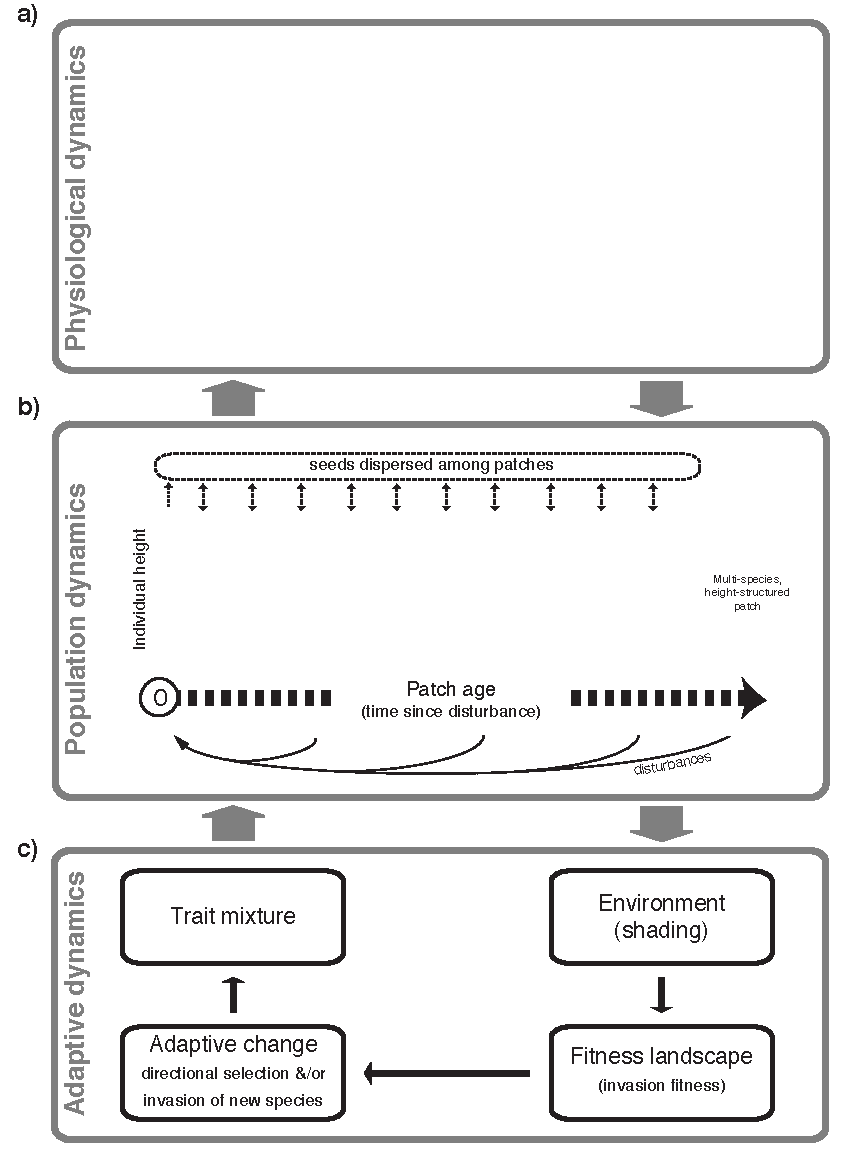
\includegraphics[height= 27cm]{vignettes/schematic-frame}};


\node[rectangle, anchor=center] at ($(middle) + (1cm, 9cm)$){
  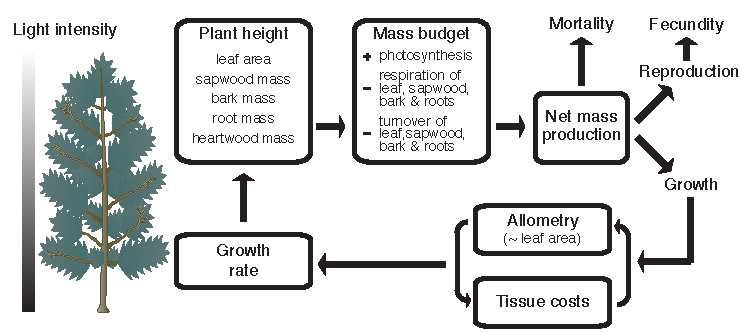
\includegraphics[width=16cm]{vignettes/schematic-phys}};


\node[rectangle, anchor=center] at ($(middle) + (0cm, -0.4cm)$){
  
\includegraphics[width=12cm]{output/middle}};

\end{tikzpicture}
\end{document}
